\documentclass[a4paper,12pt]{article} % The document class with options

\usepackage[T1]{fontenc}
\usepackage{amsmath}
\usepackage{amsfonts}
\usepackage{microtype}
\usepackage{graphicx}
\usepackage{epstopdf}
% chktex-file 1
% chktex-file 3
% chktex-file 8
% chktex-file 13
% chktex-file 18
% chktex-file 24
% chktex-file 44

\begin{document}
\setlength{\parskip}{1em} 
\setlength{\parindent}{0pt}
\newcommand{\vect}[1]{\mathbf{#1}}

\title{MECH 570C-FSI: Code Project 1 \\Fluid-structure interaction of a rigid circular cylinder}
\author{Jincong Li \\ 60539939}
\date{Feb 26th}
\maketitle

\section*{Abstract}

\section*{Introduction}
This project is designed to develop foundational knowledge in the field of fluid-structure interaction, 
focusing on a paradigmatic issue of vortex-induced vibration caused by flow around a smooth circular 
cylinder. The fluid dynamics are characterized using the incompressible, two-dimensional Navier-Stokes equations, 
formulated within the arbitrary Lagrangian-Eulerian (ALE) framework. The analysis of the rigid body structure,
which possesses a two-degree-of-freedom translational capability, is conducted employing the Lagrangian 
description. At the interface between the fluid and structure, both velocity continuity and traction 
equilibrium conditions are rigorously maintained.

\section*{Methodology}
Given that a substantial portion of the code has been provided, two primary objectives have been delineated 
as follows: The initial goal involves the execution of the IntegratedOutput function by completing the requisite 
equations to calculate the tractions and forces exerted on the cylinder's surface. The secondary task is to 
formulate the code for the Arbitrary Lagrangian-Eulerian (ALE) mesh, thereby enabling 
the accurate representation of the mesh's movement. Detailed instructions for the implementation of these 
two tasks will be elaborated upon in subsequent subsections. Moreover, the overall logic of the entire code is 
discussed in the last subsection.

\subsection*{Implementing IntegratedOutput}
The IntegratedOutput function initiates the process by identifing the indices of elements located on the cylinder's 
surface, subsequently extracting the global coordinates of each node from the matrix containing global coordinate 
information for subsequent application. Following this, the Gauss Quadrature and Galerkin Projection methods, 
in conjunction with the shape function, are applied to discretize the governing equation of the stress tensor 
along the boundary of each element on the cylinder, represented as:
\begin{align*}
    \vect{\sigma} &= -p\vect{I} + \mu(\nabla \vect{U} + \nabla \vect{U}^T),
\end{align*}
whereafter the integrals are computed for each element. The traction in x-direction ($\vect{t_x}$) is the first 
element in $\sigma$ and the traction in y-direction ($\vect{t_y}$) is the second elements. Thus the code-wise view is:
\begin{align*}
    tx(:,p) &= ((2*fluid.visc.*locgradUx-locP).*normal(:,1)\\
    & + fluid.visc.*(locgradUy+locgradVx).*normal(:,2));\\
    ty(:,p) &= ((2*fluid.visc.*locgradVy-locP).*normal(:,2)\\
    & + fluid.visc.*(locgradUy+locgradVx).*normal(:,1));
\end{align*}

The next step is to multiply those tractions for each quadrature point as well as for each element on the cylinder 
boundary with their corresponding surface area and then report the forces as the output of the IntegratedOutput function.

The verification of this objective is discussed in the Result section.

\subsection*{Implementing ALEmesh}
The alemesh function starts from initializing the ALE displacement of each nodes in the global domain and forming
the local to global map. Boundary values of ALE displacement are identified to be zero on the outter boundaries and
setted equal to the corresponding displacement on the cylinder boundary.
Then with the similar implementing strategy as shown in navierstoke function, Galerkinterms function, and Poisson 
example, the governing equation of ALE mehs displacement:
\begin{align*}
    \nabla \cdot \vect{\sigma^m} &= 0,    \in \Omega^s \\                                      
    \vect{\sigma} &= \nabla \vect{\eta} + \nabla \vect{\eta}^T + (\nabla \cdot \vect{\eta})\vect{I}
\end{align*}
is firstly transformed into weak form:
\begin{align*}
    \int_{\Omega} \left( \nabla v \cdot \nabla \eta + \nabla v \cdot (\nabla \eta)^T + (\nabla \cdot \eta)(\nabla \cdot v) \right) d\Omega = 0
\end{align*}

Then by applying the Gauss Quadrature and Galerkin Projection methods with the shape function, the corresponding terms 
are represented by stiffness matrix (please refer to the code for detail information) and the displacement for free nodes 
are solved and returned as the output of alemesh function. Note the velocity of ALE mesh movement is also computed since 
the navierstoke function requires it. 

\subsection*{Overall Logic}
The overall logic of the code is explained as follows: In each timestep in main function, the IntegratedOutput function computes the force on the cylinder surface at current location, and then 
the rigidbody function convert the forces into displacement of the cylinder boundary. ALEmesh function then computed new 
displacement for all nodes other than the outter boundaries and cylinder boundary according to the displacement of the 
cylinder boundary and compute the velocity of mesh movement. Thus, the global coordinates of each nodes are updated 
in the main function. Finally, the navierstoke function takes the updated coordinates information and mesh velocity as input,
it returns corresponding fluid velocity and pressure distribution.

In the next timestep, all information from the last timestep is stored as ``previous'' version and repeat the 
procedure indicated above. 

\section*{Results}
\subsection*{Verification of IntegratedOutput}
By setting Reynolds number to 100 (viscosity of the fluid is set to be 5 instead of 10) and disable the rigidbody function 
and alemesh function (equivalent to a stationary cylinder), the code runs for 2000 timesteps with $\varDelta  t =  0.1s$.
The following is the coefficient analysis and their plots.
\begin{table}[ht]
    \centering
    \caption{IntegratedOutput Result Comparison}
% \label{tab:Comparison of Reference Values and Simulated Values}
    \begin{tabular}{|l|c|c|}
      \hline
      \rule{0pt}{15pt}
       & Reference Values & Simulated Values \\
      \hline
      \rule{0pt}{15pt}
      $\bar C_d$ & 1.375 & 1.3753 \\
      \hline
      \rule{0pt}{15pt}
      $C_l^{\max}$ & 0.3352 & 0.3359 \\
      \hline
      \rule{0pt}{15pt}
      $\bar C_l^{rms}$ & 0.2368 & 0.2375 \\
      \hline
    \end{tabular}
  \end{table}
Since the simulated values agree with the reference values, one can conclude the implementation of the IntegratedOutput
function is correct. Also the plots of coefficient of lift and drag are shown below in Figure 1 \& 2.
\begin{figure}[htbp]
    \center
    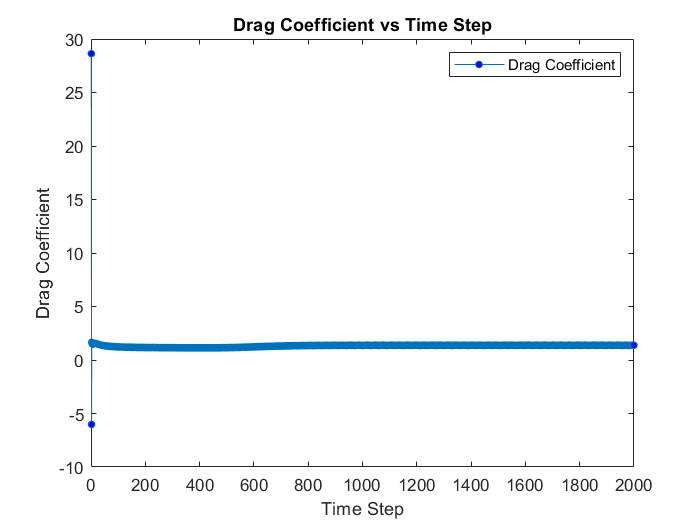
\includegraphics[scale=0.6]{Cl.png}
    \caption{Drag Coefficient}
\end{figure}
\begin{figure}[htbp]
    \center
    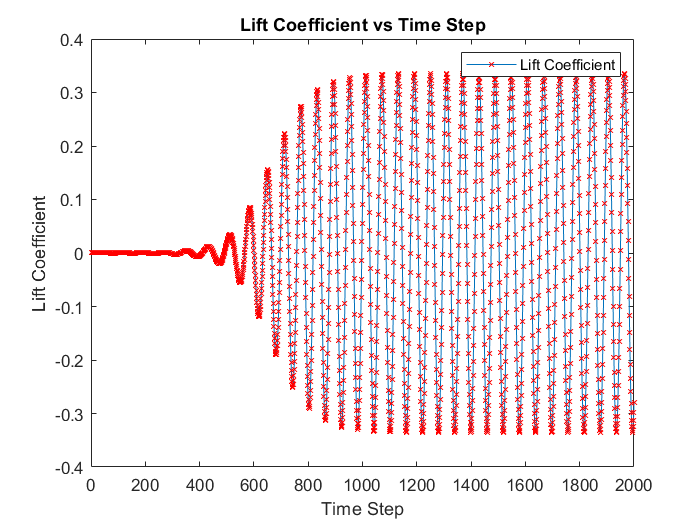
\includegraphics[scale=0.6]{Cd.png}
    \caption{Lift Coefficient}
\end{figure}

\subsection*{Verification of ALE mesh}
The alemesh function is tested by executing a simulation for a two-degree-of-freedom vortex-induced vibration (VIV)
 scenario of the cylinder, devoid of any damping coefficient, at a Reynolds number (\(Re\)) of 200, featuring a 
 mass ratio \(m^* = \frac{4m}{\rho f D^2} = 10\); and a reduced velocity \(U_r = \frac{U}{f_n D} = 5\), where 
 \(m\) denotes the mass of the cylinder, and \(f_n = \frac{\sqrt{k/m}}{2\pi}\) represents the natural frequency 
 of the elastically mounted cylinder with \(k = k_x = k_y\) being the spring stiffness. The outcomes of this 
 simulation can be compared with the results shown in the Table 2. 
 \begin{table}[ht]
    \centering
    \caption{VIV Problem Result Comparison}
% \label{tab:Comparison of Reference Values and Simulated Values}
    \begin{tabular}{|l|c|c|}
      \hline
      \rule{0pt}{15pt}
       & Reference Values\textsuperscript{[1]} & Simulated Values \\
      \hline
      \rule{0pt}{15pt}
      $\bar C_d$ & 2.0551 & 1.1369 \\
      %\hline
      %\rule{0pt}{15pt}
      %$C_l^{\max}$ & 0.3352 & 0.3359 \\
      \hline
      \rule{0pt}{15pt}
      $\bar C_l^{rms}$ & 0.0893 & 0.5062\\
      \hline
    \end{tabular}
  \end{table}
Note that the simulation of the VIV problem is not quite correct. In the simulation, the cylinder tends to flutter
after 50 seconds, so the simulated value shown in Table 2 is computed from the first 500 steps. The overall coefficients
plots are shown in Figure 3 \& 4 below.
  \begin{figure}[htbp]
    \center
    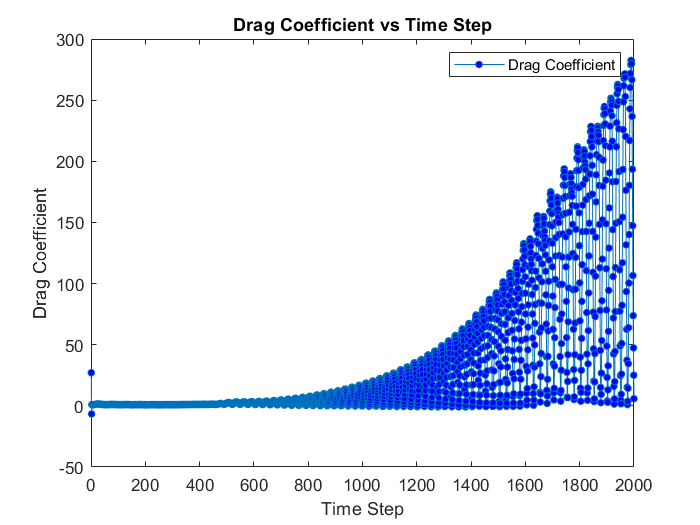
\includegraphics[scale=0.6]{Cd_1.png}
    \caption{Drag Coefficient}
\end{figure}
\begin{figure}[htbp]
    \center
    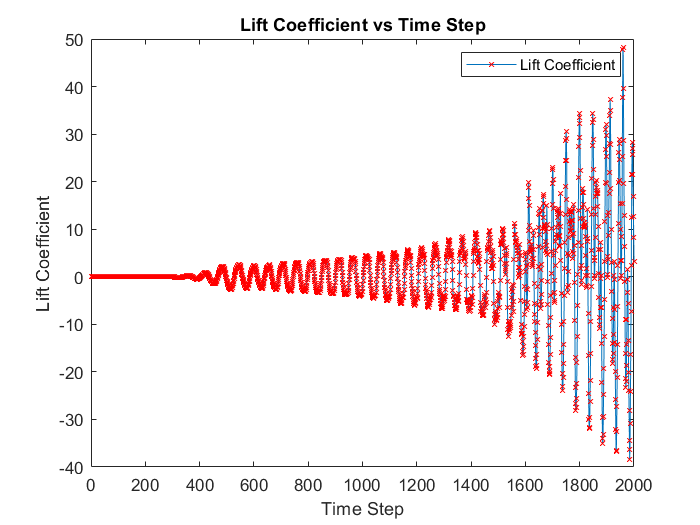
\includegraphics[scale=0.6]{Cl_1.png}
    \caption{Lift Coefficient}
\end{figure}


\section*{Conclusion}

\section*{Reference}
[1]:"On the vortex-induced oscillations of a freely vibrating cylinder in the vicinity of a stationary plane wall" L.
Zhong, W. Yao, K. Yag, R. Jaiman, B. C. Khoo, Journal of Fluids and Structures, 65, Pg. 495-526 (2016).
\end{document}